El sistema para la captación de energía undimotriz que se pretende
estudiar, funciona por medio del sistema Columna de Agua Oscilante o OWC
(\emph{Oscillating Water Column}).

Constan de una estructura parcialmente sumergida hueca por la parte de
abajo, dentro de la cual hay una cámara de aire, en algunos casos por
debajo del nivel del mar. El movimiento del oleaje se traduce en presión
sobre el aire situado en el interior, que se expansiona y comprime
accionando una turbina que a su vez acciona el generador. La turbina que
se suele instalar, está diseñada para girar en la misma dirección para
ambos sentidos del flujo, ya que posee álabes de perfil simétrico.

La estructura suele ser una cavidad cilíndrica o rectandular (con
inclinación), y a medida que se acerca a la turbina se va estrechado con
el fin de amplificar la presión y que el sistema turbina -- generador
funcione correctamente. La velocidad en la turbina es máxima cuando el
sistema entra en resonancia, es decir cuando la frecuencia natural de la
turbina y del generador coinciden con la de la ola. Los rendimientos
suelen ser del 30-50\% y pueden estar instalados en estructuras fijas o
en estructuras móviles o flotantes, o bien sobre el macizo rocoso de la
costa aprovechando instalaciones portuarias. La potencia a la que operan
oscila entre los 100 y 500 KW.

\begin{figure}
\centering
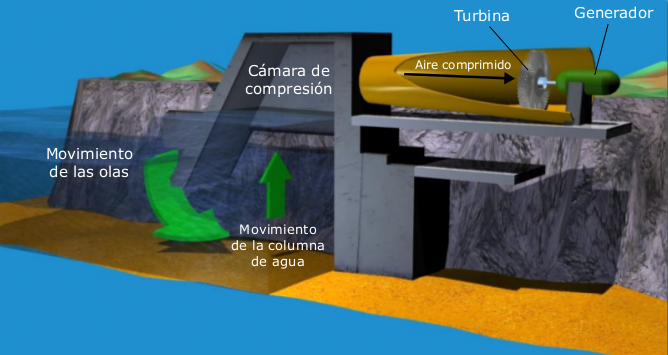
\includegraphics[width=\linewidth]{61-OWC.png}
\caption{Imagen de un convertidor de olas en energía OWC}
\end{figure}

En general todos los prototipos presentan los mismos retos tecnológicos,
entre ellos:

\begin{itemize}
\item
  Mejora de los rendimientos de las turbinas, del sistema de conversión
  hidráulica a alta presión y del funcionamiento a nivel general.
\item
  Difícil integración a la red debido a las fuertes fuctuaciones de
  potencia.
\end{itemize}
